\documentclass[a4paper]{article}
\usepackage[a4paper,margin=0mm]{geometry}
\usepackage{fontspec}
\usepackage{unicode-math}
\usepackage{tikz}
\usepackage{xcolor}
\usepackage[absolute]{textpos}
\usepackage{enumitem}
\usepackage{booktabs}
\usetikzlibrary{calc}

\setmainfont{Libertinus Serif}
\setsansfont{Libertinus Sans}
\setmathfont{Libertinus Math}

\definecolor{accent}{HTML}{F46530}
\definecolor{accentlight}{HTML}{FFEEE8}
\definecolor{ink}{HTML}{2A2E30}

\setlength{\TPHorizModule}{1mm}
\setlength{\TPVertModule}{1mm}
\pagestyle{empty}

\newcommand{\pageheader}[2]{%
\begin{textblock*}{210mm}(0mm,0mm)
  
\begin{tikzpicture}[remember picture,overlay]
    \fill[accentlight] (0,0) rectangle (210mm,14mm);
  \end{tikzpicture}
\end{textblock*}
\begin{textblock*}{60mm}(12mm,4mm)
  {\sffamily\bfseries\color{accent}\large #1}
\end{textblock*}
\begin{textblock*}{110mm}(98mm,4mm)
  \raggedleft{\sffamily\bfseries\color{accent}\large #2}
\end{textblock*}
}

\newcommand{\pagefooter}[1]{%
\begin{textblock*}{186mm}(12mm,280mm)
  \begin{tikzpicture}[remember picture,overlay]
    \draw[accent,line width=0.4pt] (0,0) -- (186mm,0);
  \end{tikzpicture}
\end{textblock*}
\begin{textblock*}{60mm}(12mm,283mm)
  {\sffamily\itshape\color{accent}\small @sat1200plus}
\end{textblock*}
\begin{textblock*}{20mm}(178mm,283mm)
  \raggedleft{\sffamily\color{accent}\small #1}
\end{textblock*}
}

\newcommand{\sectionlabel}[1]{%
\begin{textblock*}{170mm}(20mm,20mm)
{\sffamily\bfseries\itshape\Large\centering #1\par}
\end{textblock*}
}

\begin{document}

% ================= PAGE 1: CONCEPTS - Concept 1 + Concept 2 intro =================
\pageheader{LESSON 1}{ARITHMETIC \& ORDER OF OPERATIONS}
\mbox{}%
\pagefooter{1}
\sectionlabel{Concepts}

\begin{textblock*}{170mm}(20mm,32mm)
{\fontsize{11}{15}\selectfont

{\sffamily\bfseries\color{accent} 1. Arifmetik Amallar va Ularning Nomlari}

\vspace{2mm}
\emph{Qo'shish, ayirish, ko'paytirish va bo'lish kabi sonlar ustida bajariladigan harakatlar arifmetik amallar deb ataladi. Har bir amalning natijasi ham o'z nomiga ega: qo'shishning natijasi \textemdash\ yig'indi, ayirishniki \textemdash\ ayirma, ko'paytirishniki \textemdash\ ko'paytma, bo'lishniki \textemdash\ bo'linma deb ataladi.}

\vspace{1mm}
{\color{ink!70}\small Addition, subtraction, multiplication, and division are called arithmetic operations. Each result also has its own name: a sum, a difference, a product, a quotient.}

\vspace{2mm}
{\small\textbf{SAT uchun nega muhim:} bu natija-nomlari aynan SAT so'z masalalarida ishlatiladigan so'zlar \textemdash\ "the sum of $x$ and 7," "the product of two consecutive integers" \textemdash\ shuning uchun bu shunchaki atama emas, ingliz tilidan tenglamaga o'tishning birinchi qadami.}

\vspace{3mm}
\begin{center}
\small
\begin{tabular}{p{32mm}p{22mm}p{28mm}p{28mm}}
\toprule
\textbf{Amal} & \textbf{Belgi} & \textbf{Natija nomi} & \textbf{English} \\
\midrule
Qo'shish & $+$ & Yig'indi & Sum \\
Ayirish & $-$ & Ayirma & Difference \\
Ko'paytirish & $\times,\ ab$ & Ko'paytma & Product \\
Bo'lish & $\dfrac{a}{b}$ & Bo'linma & Quotient \\
\bottomrule
\end{tabular}
\end{center}

\vspace{4mm}
{\sffamily\bfseries\color{accent} 2. Amallar Bajarish Tartibi (Order of Operations)}

\vspace{2mm}
\emph{Bir nechta amalni o'z ichiga olgan ifodani hisoblashda, amallarning qat'iy belgilangan ketma-ketlikda bajarilishini talab qiluvchi qoida amallar bajarish tartibi deb ataladi: avval qavs ichidagi amallar, so'ngra daraja va ildiz, keyin II bosqich amallari \textemdash\ ko'paytirish va bo'lish (chapdan o'ngga), va eng oxirida I bosqich amallari \textemdash\ qo'shish va ayirish (chapdan o'ngga).}

\vspace{2mm}
\begin{center}
{\sffamily\bfseries\color{ink} Qavs $\;\to\;$ Daraja/ildiz $\;\to\;$ II bosqich ($\times,\div$) $\;\to\;$ I bosqich ($+,-$)}
\end{center}

\vspace{2mm}
{\small Uzbek curriculum teaches this as \emph{I bosqich} (+, $-$) and \emph{II bosqich} ($\times,\div$) rather than the English mnemonic "PEMDAS" \textemdash\ keep that native framing as the primary mental model; introduce PEMDAS only as a side-note students will recognize in imported materials.}

}
\end{textblock*}

\clearpage

% ================= PAGE 2: CONCEPTS - grouping rule, model, your-turn, mistakes, vocab =================
\pageheader{LESSON 1}{ARITHMETIC \& ORDER OF OPERATIONS}
\mbox{}%
\pagefooter{2}

\begin{textblock*}{170mm}(20mm,18mm)
{\fontsize{11}{15}\selectfont

{\small\textbf{E'tibor bering:} "qavs" bosqichi faqat ko'zga ko'ringan qavslarni emas, \textbf{kasr chizig'ini} (hammasi tepada va hammasi pastda guruhlangandek) va \textbf{modul belgisini} ($|\ |$, ichidagi amal avval bajariladi) ham o'z ichiga oladi \textemdash\ bu eng muhim SAT-ga xos kengaytma.}

\vspace{3mm}
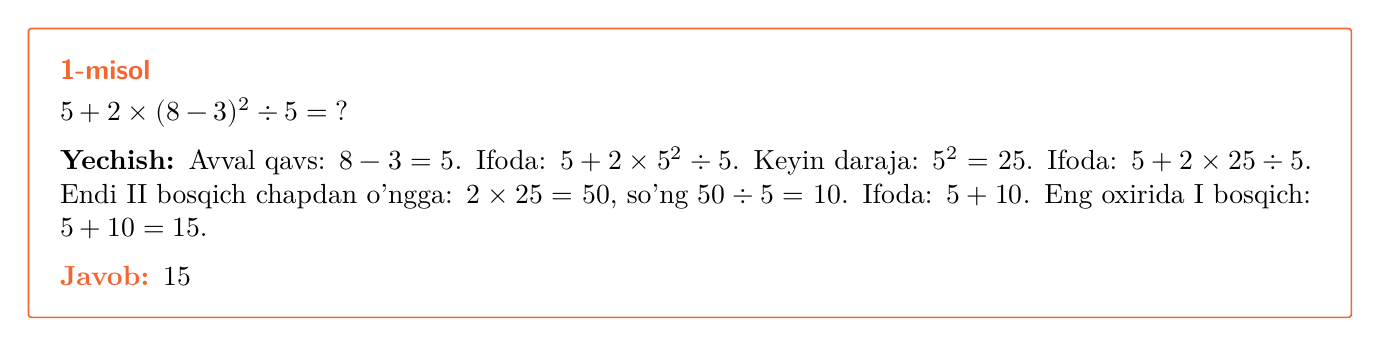
\begin{tikzpicture}
\node[draw=accent,line width=0.6pt,rounded corners=1pt,inner sep=4mm,text width=160mm,align=left] {%
{\sffamily\bfseries\color{accent} 1-misol}\\[1mm]
$5 + 2 \times (8-3)^2 \div 5 = ?$\\[2mm]
\textbf{Yechish:} Avval qavs: $8-3=5$. Ifoda: $5+2\times5^2\div5$. Keyin daraja: $5^2=25$. Ifoda: $5+2\times25\div5$. Endi II bosqich chapdan o'ngga: $2\times25=50$, so'ng $50\div5=10$. Ifoda: $5+10$. Eng oxirida I bosqich: $5+10=15$.\\[2mm]
{\color{accent}\textbf{Javob:}} $15$
};
\end{tikzpicture}

\vspace{3mm}
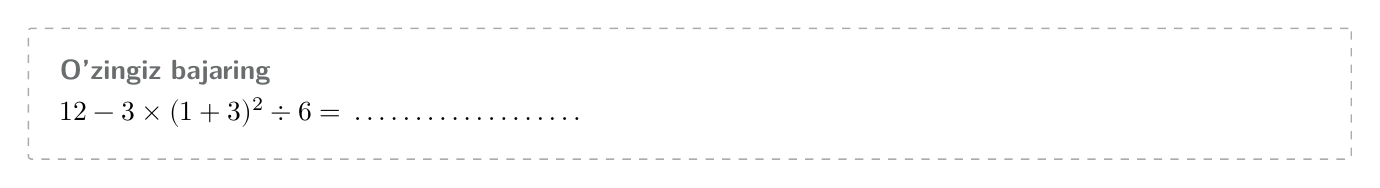
\begin{tikzpicture}
\node[draw=ink!40,line width=0.5pt,dashed,rounded corners=1pt,inner sep=4mm,text width=160mm,align=left] {%
{\sffamily\bfseries\color{ink!70} O'zingiz bajaring}\\[1mm]
$12 - 3\times(1+3)^2 \div 6 = \makebox[30mm]{\dotfill}$
};
\end{tikzpicture}

\vspace{3mm}
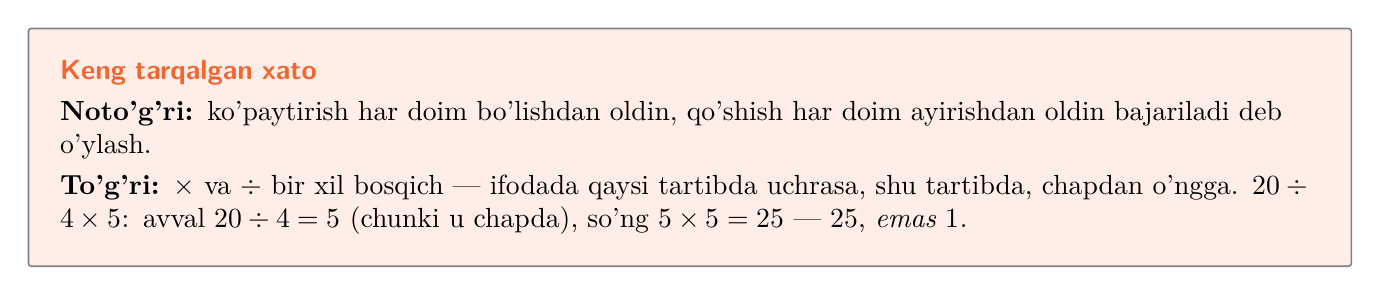
\begin{tikzpicture}
\node[draw=ink!60,line width=0.6pt,rounded corners=1pt,inner sep=4mm,text width=160mm,align=left,fill=accentlight] {%
{\sffamily\bfseries\color{accent} Keng tarqalgan xato}\\[1mm]
\textbf{Noto'g'ri:} ko'paytirish har doim bo'lishdan oldin, qo'shish har doim ayirishdan oldin bajariladi deb o'ylash.\\[1mm]
\textbf{To'g'ri:} $\times$ va $\div$ bir xil bosqich \textemdash\ ifodada qaysi tartibda uchrasa, shu tartibda, chapdan o'ngga. $20\div4\times5$: avval $20\div4=5$ (chunki u chapda), so'ng $5\times5=25$ \textemdash\ $25$, \emph{emas} $1$.
};
\end{tikzpicture}

\vspace{3mm}
\begin{center}
$\dfrac{10-4}{2\times3} \;\ne\; 10-\dfrac{4}{2}\times3 \qquad(1 \ne 4)$
\end{center}

\vspace{2mm}
{\sffamily\bfseries\small\color{accent} Vocabulary}
\vspace{1mm}

\begin{minipage}[t]{80mm}
\small
Arithmetic operation \textemdash\ Arifmetik amal\\
Sum / Difference \textemdash\ Yig'indi / Ayirma\\
Product / Quotient \textemdash\ Ko'paytma / Bo'linma\\
Order of operations \textemdash\ Amallar bajarish tartibi
\end{minipage}%
\begin{minipage}[t]{80mm}
\small
Parentheses / Exponent \textemdash\ Qavs / Daraja\\
Fraction bar \textemdash\ Kasr chizig'i\\
Absolute value bars \textemdash\ Modul belgisi\\
Left to right \textemdash\ Chapdan o'ngga
\end{minipage}

}
\end{textblock*}

\clearpage

% ================= PAGE 3: PROBLEMS - Sets 1-2 =================
\pageheader{LESSON 1}{PRACTICE}
\mbox{}%
\pagefooter{3}
\sectionlabel{Practice Sets}

\begin{textblock*}{170mm}(20mm,32mm)
{\fontsize{11}{15}\selectfont

{\sffamily\bfseries\color{accent} Set 1 \textemdash\ Pure Numeric Drill}

\vspace{2mm}
\begin{enumerate}[leftmargin=10mm,itemsep=2mm]
\item $3+4\times2$
\item $(3+4)\times2$
\item $20-6\div3$
\item $(18-6)\div3$
\item $2\times3^2$
\item $(2\times3)^2$
\item $18\div3\times2$
\item $10-2\times3+4$
\end{enumerate}

\vspace{4mm}
{\sffamily\bfseries\color{accent} Set 2 \textemdash\ Negative Numbers Present}

\vspace{2mm}
\begin{enumerate}[leftmargin=10mm,itemsep=2mm]
\item $-3+4\times2$
\item $(-3+4)\times2$
\item $5-(-2)\times3$
\item $(-2)^2\times3$
\item $-2^2\times3$
\item $10+(-4)\div2$
\item $(10+(-4))\div2$
\item $-5\times(-3)+2$
\end{enumerate}

}
\end{textblock*}

\clearpage

% ================= PAGE 4: PROBLEMS - Sets 3-4 =================
\pageheader{LESSON 1}{PRACTICE}
\mbox{}%
\pagefooter{4}

\begin{textblock*}{170mm}(20mm,18mm)
{\fontsize{11}{15}\selectfont

{\sffamily\bfseries\color{accent} Set 3 \textemdash\ Fraction Bar as a Grouping Symbol}

\vspace{2mm}
\begin{enumerate}[leftmargin=10mm,itemsep=2mm]
\item $\dfrac{3+5}{2\times2}$
\item $\dfrac{12-4}{2\times2}$
\item $\dfrac{2+3\times4}{7}$
\item $\dfrac{5^2-1}{3\times2}$
\item $\dfrac{6+2}{2+2}$
\item $\dfrac{20}{2+3}-1$
\item $\dfrac{18-6}{3\times(1+1)}$
\item $\dfrac{7+9}{4^2-12}$
\end{enumerate}

\vspace{4mm}
{\sffamily\bfseries\color{accent} Set 4 \textemdash\ Absolute Value Bars as a Grouping Symbol}

\vspace{2mm}
\begin{enumerate}[leftmargin=10mm,itemsep=2mm]
\item $|5-9|$
\item $|5-9|+3$
\item $-|5-9|$
\item $|3-7|\times2$
\item $|-3\times4|$
\item $|6-10|-|2-5|$
\item $10-|4-12|$
\item $|(-2)^2-9|$
\end{enumerate}

}
\end{textblock*}

\clearpage

% ================= PAGE 5: PROBLEMS - Set 5 + Set 6 =================
\pageheader{LESSON 1}{PRACTICE}
\mbox{}%
\pagefooter{5}

\begin{textblock*}{170mm}(20mm,18mm)
{\fontsize{11}{15}\selectfont

{\sffamily\bfseries\color{accent} Set 5 \textemdash\ Mixed, Real-Test Density}

\vspace{2mm}
\begin{enumerate}[leftmargin=10mm,itemsep=2mm]
\item $\dfrac{2^3+4}{6-4}-1$
\item $5+\dfrac{(6-2)^2}{4}$
\item $\dfrac{10-2\times3}{2^2}$
\item $3\times(4+2^2)-\dfrac{10}{2}$
\item $\dfrac{5^2-3\times5}{2+3}$
\item $2+3\times(7-2^2)$
\item $\dfrac{8+|3-7|}{2\times2}$
\item $(-3)^2+2\times(5-8)$
\end{enumerate}

\vspace{4mm}
{\sffamily\bfseries\color{accent} Set 6 \textemdash\ Spot the Error}

\vspace{1mm}
{\small Har bir misolda aynan bitta xato qadam bor. Qaysi qadam xato va nega, ayting, so'ng to'g'ri javobni toping.}

\vspace{2mm}
\begin{enumerate}[leftmargin=10mm,itemsep=2mm]
\small
\item $20\div4\times5$ \textemdash\ \emph{"1-qadam: $4\times5=20$. 2-qadam: $20\div20=1$."}
\item $15-3+4$ \textemdash\ \emph{"1-qadam: $3+4=7$. 2-qadam: $15-7=8$."}
\item $\dfrac{10+2}{2\times3}$ \textemdash\ \emph{"Avval $2\times3=6$, so'ng $2\div6=\frac13$, so'ng $10+\frac13$."}
\item $-4^2$ \textemdash\ \emph{"$-4^2=(-4)^2=16$."}
\item $3-|5-9|$ \textemdash\ \emph{"$3-5-9=-11$."}
\end{enumerate}

}
\end{textblock*}

\clearpage

% ================= PAGE 6: PROBLEMS - Set 7 + Answer Key =================
\pageheader{LESSON 1}{PRACTICE}
\mbox{}%
\pagefooter{6}

\begin{textblock*}{170mm}(20mm,18mm)
{\fontsize{11}{15}\selectfont

{\sffamily\bfseries\color{accent} Set 7 \textemdash\ Bonus / Challenge (\textasciitilde90 sec each)}

\vspace{2mm}
\begin{enumerate}[leftmargin=10mm,itemsep=2mm]
\item $|(-3)^2-2\times(5-8)|\div3$
\item $\dfrac{4+|2-6|^2}{3\times2-2}$
\item $2\times\left[(10-4)^2\div3+1\right]-5$
\item $\dfrac{|-12|+3^2}{7-4}$
\item $1+2\times\left[|4-10|-(3-1)^2\right]$
\end{enumerate}

\vspace{5mm}
{\sffamily\bfseries\small\color{accent} Answer Key}
\vspace{1mm}

\begin{minipage}[t]{80mm}
\small
\textbf{Set 1:} 11, 14, 18, 4, 18, 36, 12, 8\\[1mm]
\textbf{Set 2:} 5, 2, 11, 12, $-12$, 8, 3, 17\\[1mm]
\textbf{Set 3:} 2, 2, 2, 4, 2, 3, 2, 4\\[1mm]
\textbf{Set 4:} 4, 7, $-4$, 8, 12, 1, 2, 5
\end{minipage}%
\begin{minipage}[t]{80mm}
\small
\textbf{Set 5:} 5, 9, 1, 19, 2, 11, 3, 3\\[1mm]
\textbf{Set 6:} 25, 16, 2, $-16$, $-1$\\[1mm]
\textbf{Set 7:} 5, 5, 21, 7, 5
\end{minipage}

}
\end{textblock*}

\end{document}
